
\capitulo{3}{Conceptos teóricos}\label{cap:Conceptos teóricos}

Este punto nace ante la necesidad de enmarcar el proyecto dentro de las tecnologías y elementos que utilizaremos durante todo el proyecto y que no tienen por qué conocerse.

El término `domótica’ es el pilar principal del proyecto y, por ello, comenzaré explicando lo qué es y cómo lo enfocaremos:

\section{Domótica}\label{concepto:Domótica}
La domótica podemos definirla como aquel conjunto de elementos capaces de automatizar una vivienda aportando un beneficio.
En nuestro caso, el sistema domótico deberá controlar luces, persianas y calefacción permitiendo un aumento del confort y la seguridad, además de permitir un consumo eficiente de recursos a la hora de climatizar la vivienda.

\begin{displayquote}
\Chapter{\textit{The home automation system can be applied to many areas including home security, lighting control, flame detection, smart heating, motion sensor and door control to provides its homeowner's comfort, security, energy efficiency (low operating costs) and convenience at all times. The Internet of Things (IoT) is anticipated to enable a variety of smart home services in which each service provides a set of home automation solutions. This proposed study consists of developing an automated home monitoring using Raspberry Pi that provides a customizable and cost-efficient platform for a smart home.}} \cite{inproceedings:CitaDomotica}
\end{displayquote}

\section{GPIO}\label{concepto:GPIO}
Éstos son unos puertos de entrada y salida conformados en forma de pines que están albergados en las placas Raspberry Pi~\cite{misc:RbPWeb}, al igual que en todos los microcontroladores~\cite{misc:descubrearduino}. Los puertos GPIO, de por sí, únicamente intercambian información entre dispositivos en forma de señales digitales, pero sin una funcionalidad específica. En el presente proyecto, gracias a ellos, enviaremos órdenes a otros dispositivos externos para que realicen las tareas que les designemos, como controlar unos relés para conseguir la acción final de subir o bajar una persiana.

Existen tres tipos de puertos GPIO en Raspberry Pi

Podemos ver los GPIO de la Raspberry Pi en la imagen~\ref{Img:3.RaspberryPi}~\footnote{Imagen original de ~\url{https://raspberryparatorpes.net/ }}, y también, la imagen~\ref{Img:3.GPIOReadAll} del comando <<gpio readall>> dentro de RasperryPi OS, donde podemos ver las numeraciones física, BCM y GPIO de los pines de la placa.

\begin{figure}
    \centering
    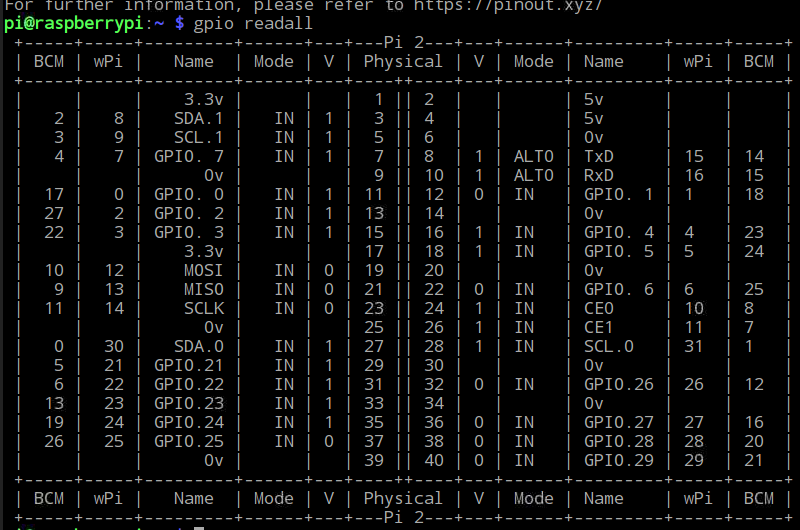
\includegraphics[width=.9\textwidth]{img/fotos/gpioReadall.png}
    \caption[Salida comando gpio readall]{Salida comando gpio readall.} \label{Img:3.GPIOReadAll}
\end{figure}

\begin{figure}
    \centering
    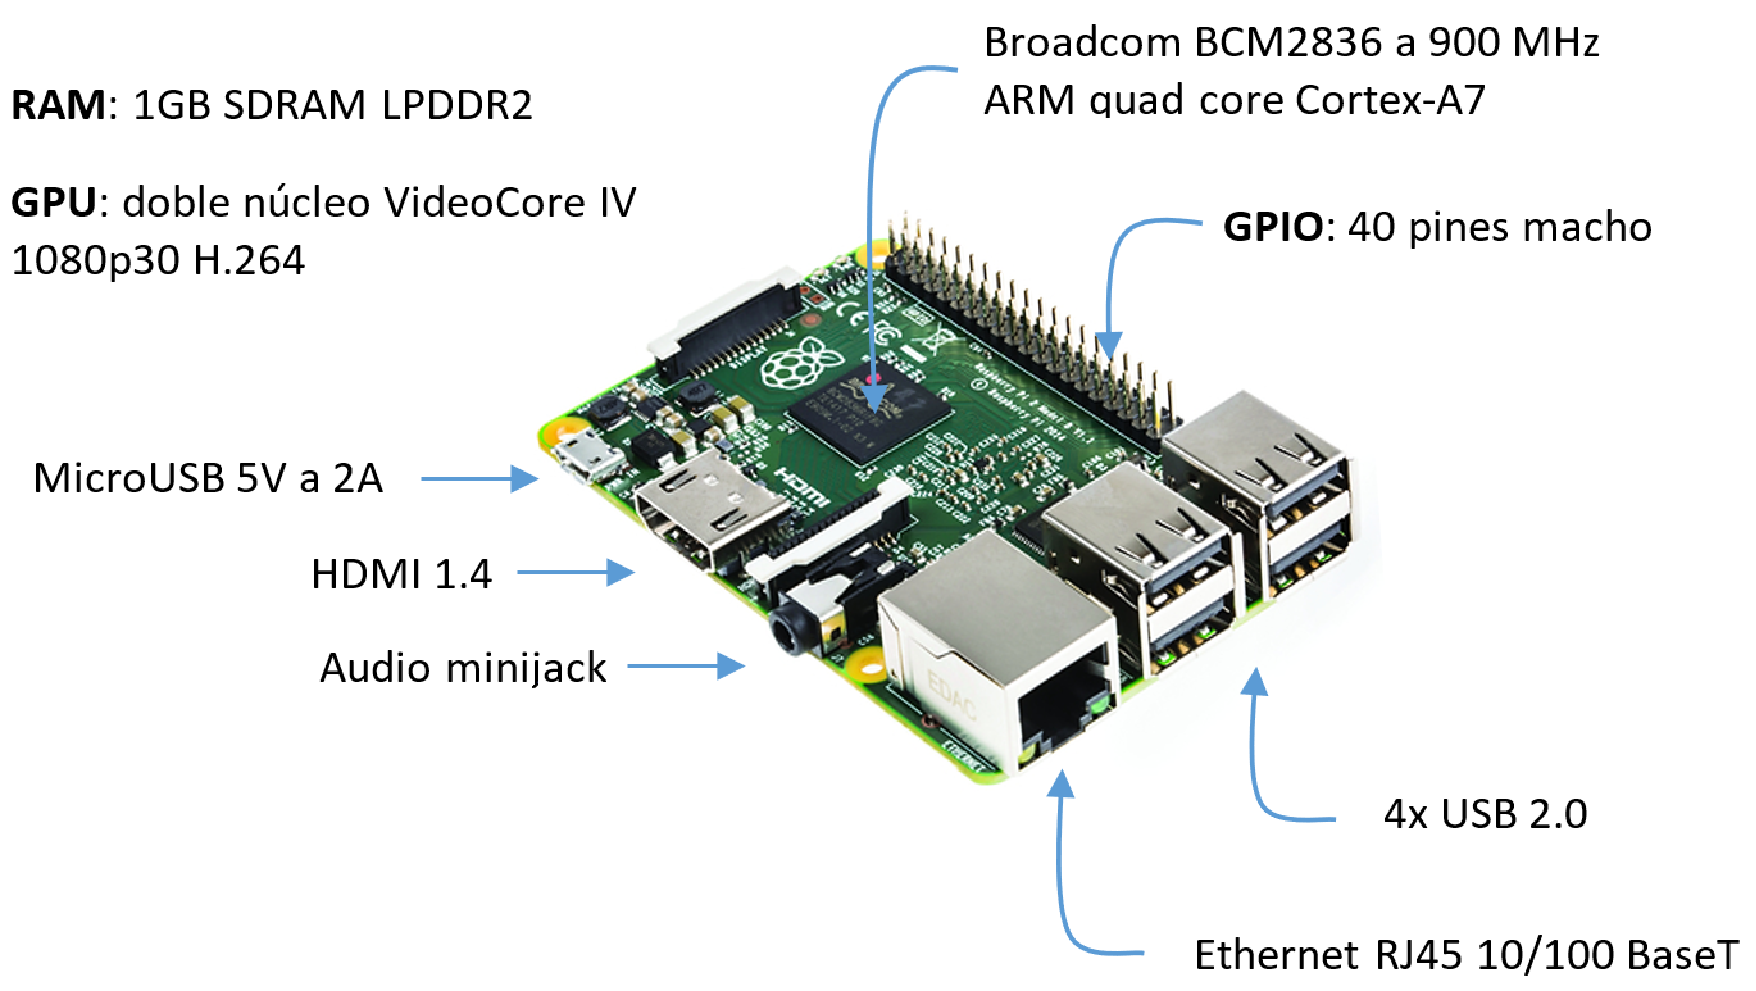
\includegraphics[width=.9\textwidth]{img/RBP2B.pdf}
    \caption[Componentes Raspberry Pi]{Componentes Raspberry Pi.} \label{Img:3.RaspberryPi}
\end{figure}

\section{API}\label{concepto:API}
Es el acrónimo de ‘Application Programming Interfaces’ que, traducido al castellano significa ‘Interfaz de Programación de Aplicaciones’. Estas interfaces nos sirven para realizar desarrollos. En nuestro caso utilizamos la información obtenida de Latitud y Longitud así como las temperaturas del día siguiente.
En el proyecto, accedemos a una URL como esta ~\url{http://ip-api.com/json/?fields=country,regionName,city,lat,lon,isp,query}, obteniendo los valores de país, región, ciudad, latitud, longitud, ISP y dirección IP.
Estos valores, podemos recogerlos directamente desde Python en formato json~\cite{misc:Json}~\ref{4:JSON}.

Otro ejemplo de API podemos verlo en Telegram, ya que utilizaremos su API orientada a crear bots para poder interactuar con nuestro sistema domótico. Podemos ver como funciona la API de Telegram con un bot programado por nosotros dependiendo de una Raspberry Pi en la imagen~\ref{Img:3.FuncionamientoBot}, que es la misma arquitectura que se ha utilizado en el proyecto.

\begin{figure}
    \centering
    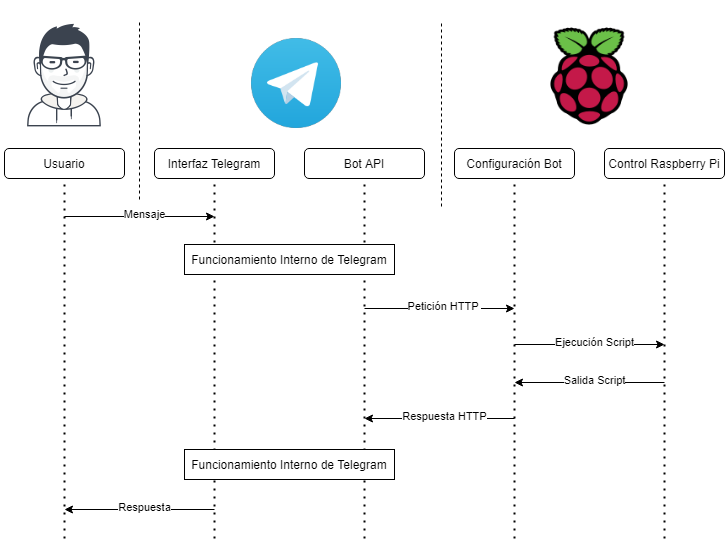
\includegraphics[width=1.\textwidth]{img/Diagramas/FuncionamientoBot.png}
    \caption[Funcionamiento Bot]{Funcionamiento Bot de Telegram con Raspberry Pi.} \label{Img:3.FuncionamientoBot}
\end{figure}

\section{Telegram}\label{concepto:Telegram}
Telegram es una aplicación de mensajería multiplataforma. Esta plataforma dispone de APIs a disposición de los usuarios que éstos pueden programar y poner a su propia disposición.
Podemos visitar la página web de la aplicación de mensajería en~\url{https://telegram.org/}.

\subsection{Bot de Telegram}\label{concepto:botTelegram}
Un bot, es un programa que permite simular una conversación en ciertos aspectos. Uno de estos aspectos puede ser enviarle órdenes para que las ejecute o nos brinde información de algún tipo. Como ejemplo, podemos ver plasmados ambos ejemplos en el bot que se ha desarrollado para el presente proyecto: podemos solicitarle al bot que ejecute acciones como el recopilado de datos o el envío de órdenes a los periféricos; y también que nos envíe información como puede ser una tabla informativa con las temperaturas por horas del día siguiente.

\section{Json}\label{concepto:JSON}
{Json~\cite{misc:Json}}, es el acrónimo en inglés de ‘JavaScript Object Notation’ y es un formato específico del que nos servimos para almacenar la información de forma estructurada mediante etiquetas <<key>> y etiquetas <<value>> del siguiente modo:

\begin{lstlisting}[language=json,firstnumber=0]
{
    "country":"Spain", 
    "regionName":"Madrid", 
    "city":"Getafe"
}
\end{lstlisting}

En ella, podemos ver que las etiquetas <<key>> son las que están a la izquierda de los dos puntos y las etiquetas de la derecha son las <<value>>. Tenemos un ejemplo real en el punto \ref{5.TelegramBot} del presente proyecto.

\section{RETB}\label{concepto:RETB}
Es el acrónimo de Reglamento electrotécnico para baja tensión y en él se recoge la normativa eléctrica aplicable en domicilios.
Esta norma acaba de ser actualizada y podemos disponer de la información en páginas oficiales como puede ser el BOE~\cite{manual:REBT}.
Del documento ICT-BT-21~\cite{manual:ICT-BT-21} podemos extraer información para realizar las instalaciones eléctricas de nuestro sistema domótico como el número máximo de cables a introducir por un tubo eléctrico.

\section{Normativa de ICT}\label{concepto:Normativa_ICT}
Como figura en el \textit{BOE 143, de 16 de junio de 2011, El Reglamento regulador de las infraestructuras comunes de telecomunicaciones para el acceso a los servicios de telecomunicación en el interior de las edificaciones, aprobado por el Real Decreto 346/2011, de 11 de marzo}:
Debemos regirnos por esta normativa a la hora de hacer cualquier instalación de comunicaciones nueva dentro de domicilios.
Podemos informarnos y ampliar información en la publicación en la sección de ICT en el BOE~\cite{manual:ICT}.

Por otro lado, disponemos de guías para instaladores con dibujos y tablas que facilitan la comprensión, como puede ser la documentación que publica Televés~\cite{manual:ICT-Televes}. De este punto, obtendremos la norma para introducir cableado ICT~\cite{manual:ICT} conforme a norma.

Tras hacer un estudio en mi domicilio, no necesitaré utilizar la normativa de ICT~\cite{manual:ICT} porque toda la instalación se realizará mediante canales eléctricos, pero está bien conocer la norma para, en caso de necesitarla, poder hacer uso de ella correctamente.

\section{Cableado estructurado}\label{concepto:Cableado_estructurado}
El establecimiento de un sistema de cableado estructurado consiste en la organización de los cables en un recinto conforme a una norma y constituye el nivel básico de cualquier red de comunicaciones.
Al contar y cumplir con este estándar nos damos cuenta de que tendremos instalaciones limpias, uniformes, seguras y escalables, facilitando la supervisión, el mantenimiento y posibles migraciones de tecnologías.
Un sistema de cableado genérico dispone de tres subsistemas, Troncal, de Edificio y Horizontal. En nuestro proyecto únicamente trataremos con el subsistema horizontal.

En este proyecto no contaremos con un gran número de cables, pero no está de más realizar una instalación lo más correctamente posible con unas normas de referencia

\section{WiFi}\label{concepto:WIFI}
Es una tecnología de comunicaciones de forma inalámbrica o “Wireless”. WiFi es el acrónimo traducido de <<Fidelidad Inalámbrica>> que procede del inglés <<Wireless Fidelity>>.
Estas tecnologías inalámbricas se rigen por la norma \underline{IEEE 802.11}~\cite{manual:IEEE802.11}.
En la web oficial del organismo podremos comprobar qué estándares dentro del 802.11 están vigentes y cuáles no.

\section{Tipos de cableado de datos}\label{concepto:UTP}
Es un tipo de cableado de datos que se compone de 4 pares de cables sin apantallar que están albergados dentro de una camisa de PVC, ver imagen~\ref{Img:Bobina UTP}~\footnote{Imagen original de \url{https://solarmat.es}~\cite{wiki:Creative}}.

\begin{figure}
    \centering
    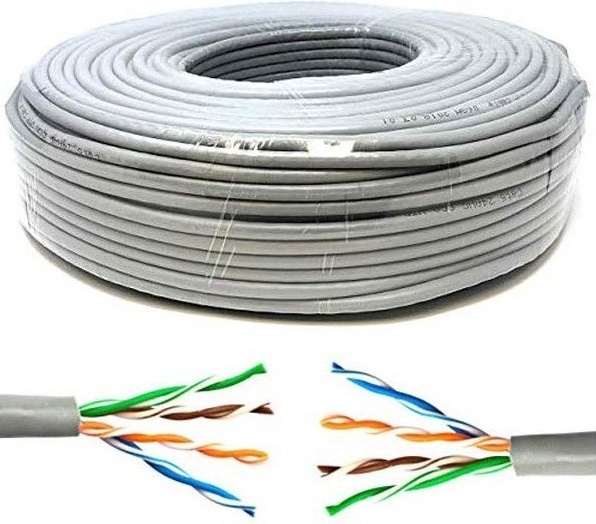
\includegraphics[width=.4\textwidth]{img/bobina.jpg}
    \caption[Bobina UTP]{Bobina UTP con muestra del mismo con corte de camisa exterior.} \label{Img:Bobina UTP}
    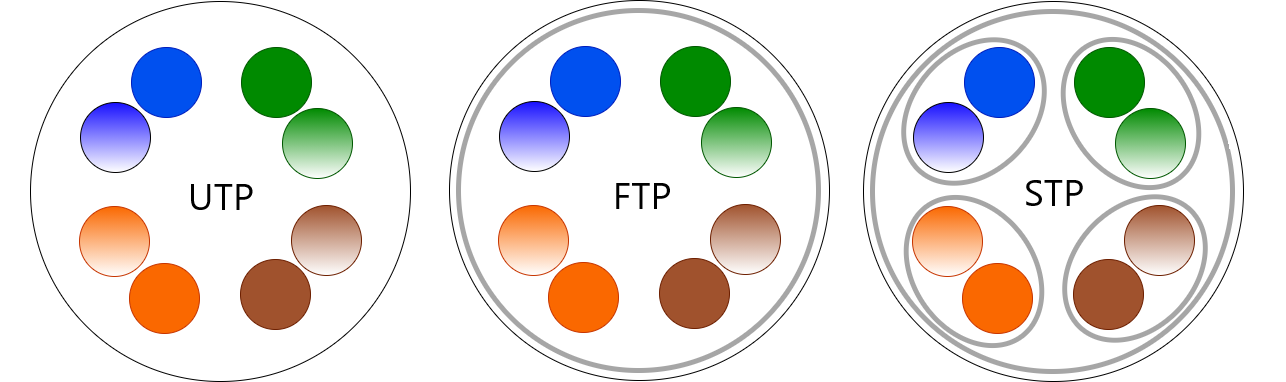
\includegraphics[width=0.9\textwidth]{img/CABLES.png}
    \caption{Diagrama de muestra de cables de datos} \label{Img:CablesDatos}
\end{figure}

Existen diferentes tipos de cables de datos: UTP, STP, FTP:
\begin{itemize}
\item Los cables \textbf{UTP} (del ingles <<Unshielded Twisted Pair>> o <<Par trenzado no apantallado>>) no disponen de protección ante interferencias electromagnéticas. Ver imagen~\ref{Img:CablesDatos}.



\item Los cables \textbf{FTP}(del inglés <<Foiled Twisted Pair>> o <<Par trenzado con pantalla global>>) disponen de una pantalla global contra interferencias electromagnéticas dentro de la camisa de PVC que recoge los 4 pares destinados a transmisión de datos. Ver imagen~\ref{Img:CablesDatos}.



\item Los cables \textbf{STP}(del inglés <<Shielded Twisted Pair>> o <<Par trenzado apantallado>>) disponen de una pantalla contra interferencias electromagnéticas por cada par de cables pero, además, también cuentan con una malla metálica exterior. Ver imagen~\ref{Img:CablesDatos}.


\end{itemize}
En nuestro caso utilizaremos UTP puesto que no necesitamos un apantallamiento ya que no transmitiremos datos y tampoco tendremos un alto grado de interferencias.
